\documentclass{article}

% AMS math symbols
\usepackage{amsfonts}
\usepackage{amsmath}
\usepackage{amssymb}

% colored textare that buyers
\usepackage{color}

% Evolutional algorithms journal template
\usepackage{ecj}

% custom enumerates
\usepackage{enumitem}

% eps figures
\usepackage[pdftex]{graphicx}

% boxed figures
\usepackage{float}

% set page margins
\usepackage[top=1in, bottom=1in, left=1in, right=1in]{geometry}

% citations with author
\usepackage{natbib}

% additional colors
\usepackage[usenames,dvipsnames]{xcolor}

\newcommand{\concat}{\ensuremath{+\!\!\!\!+\,}}
\newcommand{\usman}{\textcolor{Red}{\textbf{*** USMAN ***} }}
\newcommand{\claudio}{\textcolor{Cerulean}{\textbf{*** CLAUDIO ***} }}

%\floatstyle{boxed} 
%\restylefloat{figure}

\setlength{\parskip}{7pt}
\setlength{\parsep}{0pt}
\setlength{\parindent}{0pt}

\setlist{nolistsep}

% ADDING A FIGURE
%\begin{figure}[t]
%\begin{center}
%\psfig{file=Bsimilar.eps,width=300pt}
%\end{center}
%\caption{NKY algorithm: performance of different implementations.}
%\label{fig:Bsimilar}
%\end{figure}
%

% CITING
% \citep{citation}

\begin{document}

% uncomment this to get journal footers
%\ecjHeader{x}{x}{xxx-xxx}{200X}{genetic vs deterministic algorithms for LCS}{C.A. Andreoni, U. Masood}
\title{Caching Fractal B+ Trees}

\author{\name{\bf Claudio Alberto Andreoni} \hfill \addr{caa@mit.edu}\\ 
        \addr{Department of Mathematics, Massachusetts Institute of Technology, 
        Cambridge, 02139, United States}
\AND
       \name{\bf Usman Masood} \hfill \addr{usmanm@mit.edu}\\
        \addr{Department of Electrical Engineering and Computer Science,
Massachusetts Institute of Technology, 
        Cambridge, 02139, United States}
}

\maketitle

\begin{abstract}
The two primary requirements for database systems are handling data queries
rapidly and utilizing storage thriftily.
However, these often stand in contrast with each other,
as traditionally space usage and achievable performance are inversely
proportional.
In order to quickly retrieve data,
databases maintain an index of searchable keys, along with the location of the
corresponding data on drive.
Modern systems such as IBM DB2, Oracle, and MS SQL Server use B+ trees for the
indexes,
due to their ability to efficiently exploit disk bandwidth \citep{Gehrke:2002}.

Fractal B+ trees (fpB+ trees), a kind of recursive B+ tree structure, were
proposed to improve performance
by adapting to both disk layout and processor cache.
However, these either increase the amount of space wasted in representing the
index,
or require an aggressive memory management scheme \citep{Chen:2002}.

We propose a new data structure named Caching Fractal B+ trees (cfB+ trees),
which replicates the structure
of fpB+ trees, but takes advantage of the wasted space to perform online caching
of database entries.
cfB+ trees simplify the complexity associated with performing index operations,
and reduce in expectation the number of reads from disk necessary to retrieve
the queried data. 
\end{abstract}

\section{Introduction}

One of the key aspects of database design is that resources, especially disk
bandwidth and memory, must be utilized efficiently. To utilize memory
efficiently, databases cache \textit{hot} tuples (most frequently accessed) in
memory so that when querying for them, they can be fetched directly from memory
rather than having to access the disk. To utilize disk bandwidth efficiently,
databases try to minimze the amount of disk pages read and perform sequential
access to disk when possible. Disks are usually an order of magnitude slower
than memory, and since data in databases needs to be persistently stored on
disk, disk bandwidth tends to be the bottleneck for practically all workload.

To accomplish the aforementioned targets, databases often employ index
structures over certain \textit{columns} to store tuple pointers so that they
can be looked up in a way faster than scanning the entire relation. As long as
the cost of reading the entire relation is less than the cost of searching for
an item in the index structure and fetching a single tuple from disk, we should
expect a performance improvement. In practice, all relations are large enough
that index structures are helpful rather than detrimental to performance.

The index structures are filled with key-value pairs, where the key is the tuple
column that we intend to search by,
and the value is a pointer to the location of the tuple on disk.
As operations are executed on the database, the index is updated
correspondingly.
This way, searches can be conducted by probing the index and then accessing the
drive using the pointer retrieved from the index.


\subsection{B+ tree Indexes}
The index structure should provide operations such as insertion, deletion,
search and in most cases range scan. B+ trees are a natural choice for index
structures because they provide all the required operations and they can be
optimized to exploit disk bandwidth efficiently. Sometimes hash tables are also
used to index data, but since they do not support range queries, they can only
be used to index columns over which range queries are never performed.
More recently othere structures of different complexity have been considered for
indexing, both cache-oblivious and cache-aware.
These however have not yet reached the same industry acceptance as B+ trees,
which are currently considered the industry standard.



\subsubsection{Optimizing B+ trees for Disk Performance}

To optimize I/O performance, traditional \textit{disk optimized} B+ trees are
composed of nodes the size equal to a \textit{disk page} -- the natural transfer
size for reading and writing to disk, traditionally 4096B.
Nodes of such sizes have room for hundreds of entries, meaninig that the
branching factor for these trees is usually quite large.
This implies that the height of the tree is rather small. This is beneficial
because only a few pages need to be read from disk in order to find the tuple
pointer we are searching for. At the same time, however, this also means that
the additional page access to retrieve the associated tuple data is a
significant part of the total cost. Typical index fill factors have been shown
to be around 68\%, which is a conscious decision to ensure that in the presence
of inserts we do not have too many expensive node split operations
\citep{Wu:2011}. A major contribution of this paper is providing a scheme to
utilize this wasted space as a tuple cache, so that for hot tuples we can read
the data directly from the leaf node page and avoid the additional disk page
access we talked about earlier needed to reading tuple data.

A downside of using traditional \textit{disk optimized} B+ trees is that they
have poor processor cache performance. They incur an excessive number of cache
misses, wasting time and forcing the eviction of useful data from the cache in
the process. This is because of the large discrepancy in node sizes and width of
cache lines -- the natural size of reading and writing to main memory. A single
cache line is usually 32B-128B wide and so the \textit{jumps} in a 4KB address
space while binary searching a node result in a lot of cache misses.
Cache prefetching, the pre-retrieval of memory entries for future usage that
modern processors feature, 
is helpful only when the range of the binary search becomes considerably small:
in that case, the processor can reduce time spent on memory reads by guessing
which future memory entries will be
read and fetch them in advance.

\subsubsection{Optimizing B+ trees for Cache Performance}

Recently, many studies have presented new types of B+ trees --
\textit{cache-sensitive B+ trees}, \textit{prefetching B+ trees} -- optimized
for cache performance \citep{Rao:2000}, \citep{Chen:2001}. These data structures
try to minimize the impact of cache misses by making node sizes equal to the
width of a cache line (or some small multiple of it). However, this technique
for cache optimization is at odds with disk performance. Small nodes result in a
small branching factor, which increases the height of the tree.
In the worst case, this results in a disk page access for each node traveled in
the search.

Fractal Prefetching B+ trees (fpB+ trees) are a type of B+ tree which try to
optimize both disk and cache performance. In this paper, we propose Caching
Fractal B+ trees (cfB+ trees) which extend fpB+ trees, in particular
\textit{disk-first} fpB+ trees, to improve cache performance further while
ensuring comparable disk performance.

\section{Fractal B+ trees}

fpB+ trees have a self-similar ``tree within a tree'' structure, as illustrated
in Figure \ref{fig:fb+tree_struct}. It is an index structure which can be viewed
at two granularities. At the outer tree level, it consists of disk-optimized
nodes (``big nodes'') with sizes roughly equal to that of disk page. At the inner tree level, it
consists of cache-optimized nodes (``small nodes'') that are roughly the size of a cache line.

\begin{figure}[h]
\begin{center}
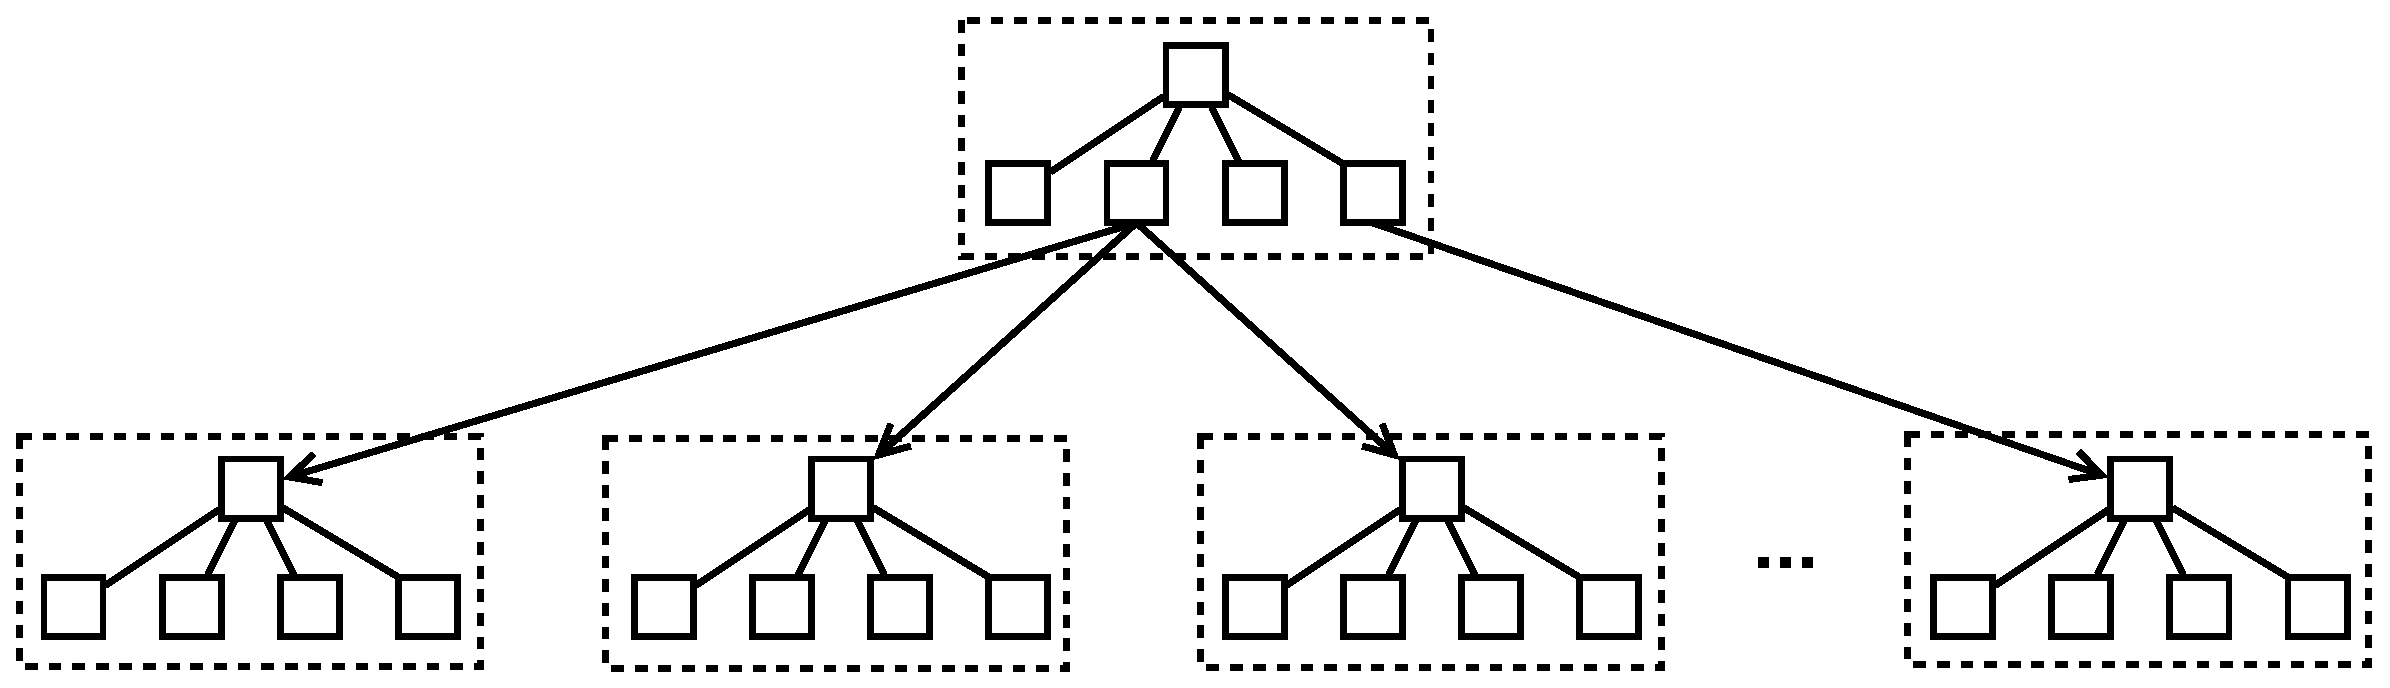
\includegraphics[width=350pt]{fb+tree_struct}
\end{center}
\caption{
Self-similar "tree within a tree" structure of fpB+ trees
}
\label{fig:fb+tree_struct}
\end{figure}

In the \textit{disk-first} variant of fpB+ trees, we start with a disk-optimized
B+ tree and then try to organize keys and pointers within each node into a
cache-optimized B+ tree. Hence, the size of nodes of the outer tree
is fixed to 4KB. The inner tree is composed of nodes that are
aligned at cache line boundaries and have sizes equal to some small multiple
of the cache line width. Both these schemes aid cache performance. In order to
pack more keys and values into the inner tree, the small non-leaf nodes use
short in-page offsets (2B) rather than full pointers (4B) because they only need
to address a 4K address range. Small leaf nodes, however, need to store full
pointers because they point to big nodes.

\subsection{Determining the Size of Small Nodes}

There is an optimal small node size determined by the architecture's memory subsystem as well as key
and pointer sizes. The optimal big node size is determined by the disk page size.
It is likely that these sizes mismatch, in the sense that an
inner tree of $k$ levels underflows a big node, and an inner tree of $k+1$ levels
overflows the big node (Figure \ref{fig:node_mismatch}). We want to pick the size of
the small nodes such that it minimizes the amount of both the unused space and the space
taken by small inner nodes, while minimizing the cost of searching through the
inner tree. 

We note that there are two parameters that affect these goals: $w$
the number of cache lines a small node spans, and $n$ the number of key/value
pairs we can fit in a single cache line. 
The branching factor of the inner tree is $b=wn = O(w)$, which makes the height
$h$ of the tree roughly equal to $\log_b N$, where $N$ is the maximum number of
items that can be indexed by a small tree. The size $s$ of a small node clearly grows
linearly with the branching factor $b$. On the other hand, the number of small inner
nodes grows roughly as $\displaystyle O\left(\frac{N}{b^2}\right)$, i.e.\ it decreases quadratically with the
branching factor. The unused space $\delta$ in a node is approximately equal to
$\displaystyle \left(4\text{KB} - \frac{1-s^{h+1}}{1-s}\right)$. Thus for better space utilization, we must try
to maximize the branching factor, which in turn implies that we must increase the
number of cache lines a small node uses.

\begin{figure}[h]
\begin{center}
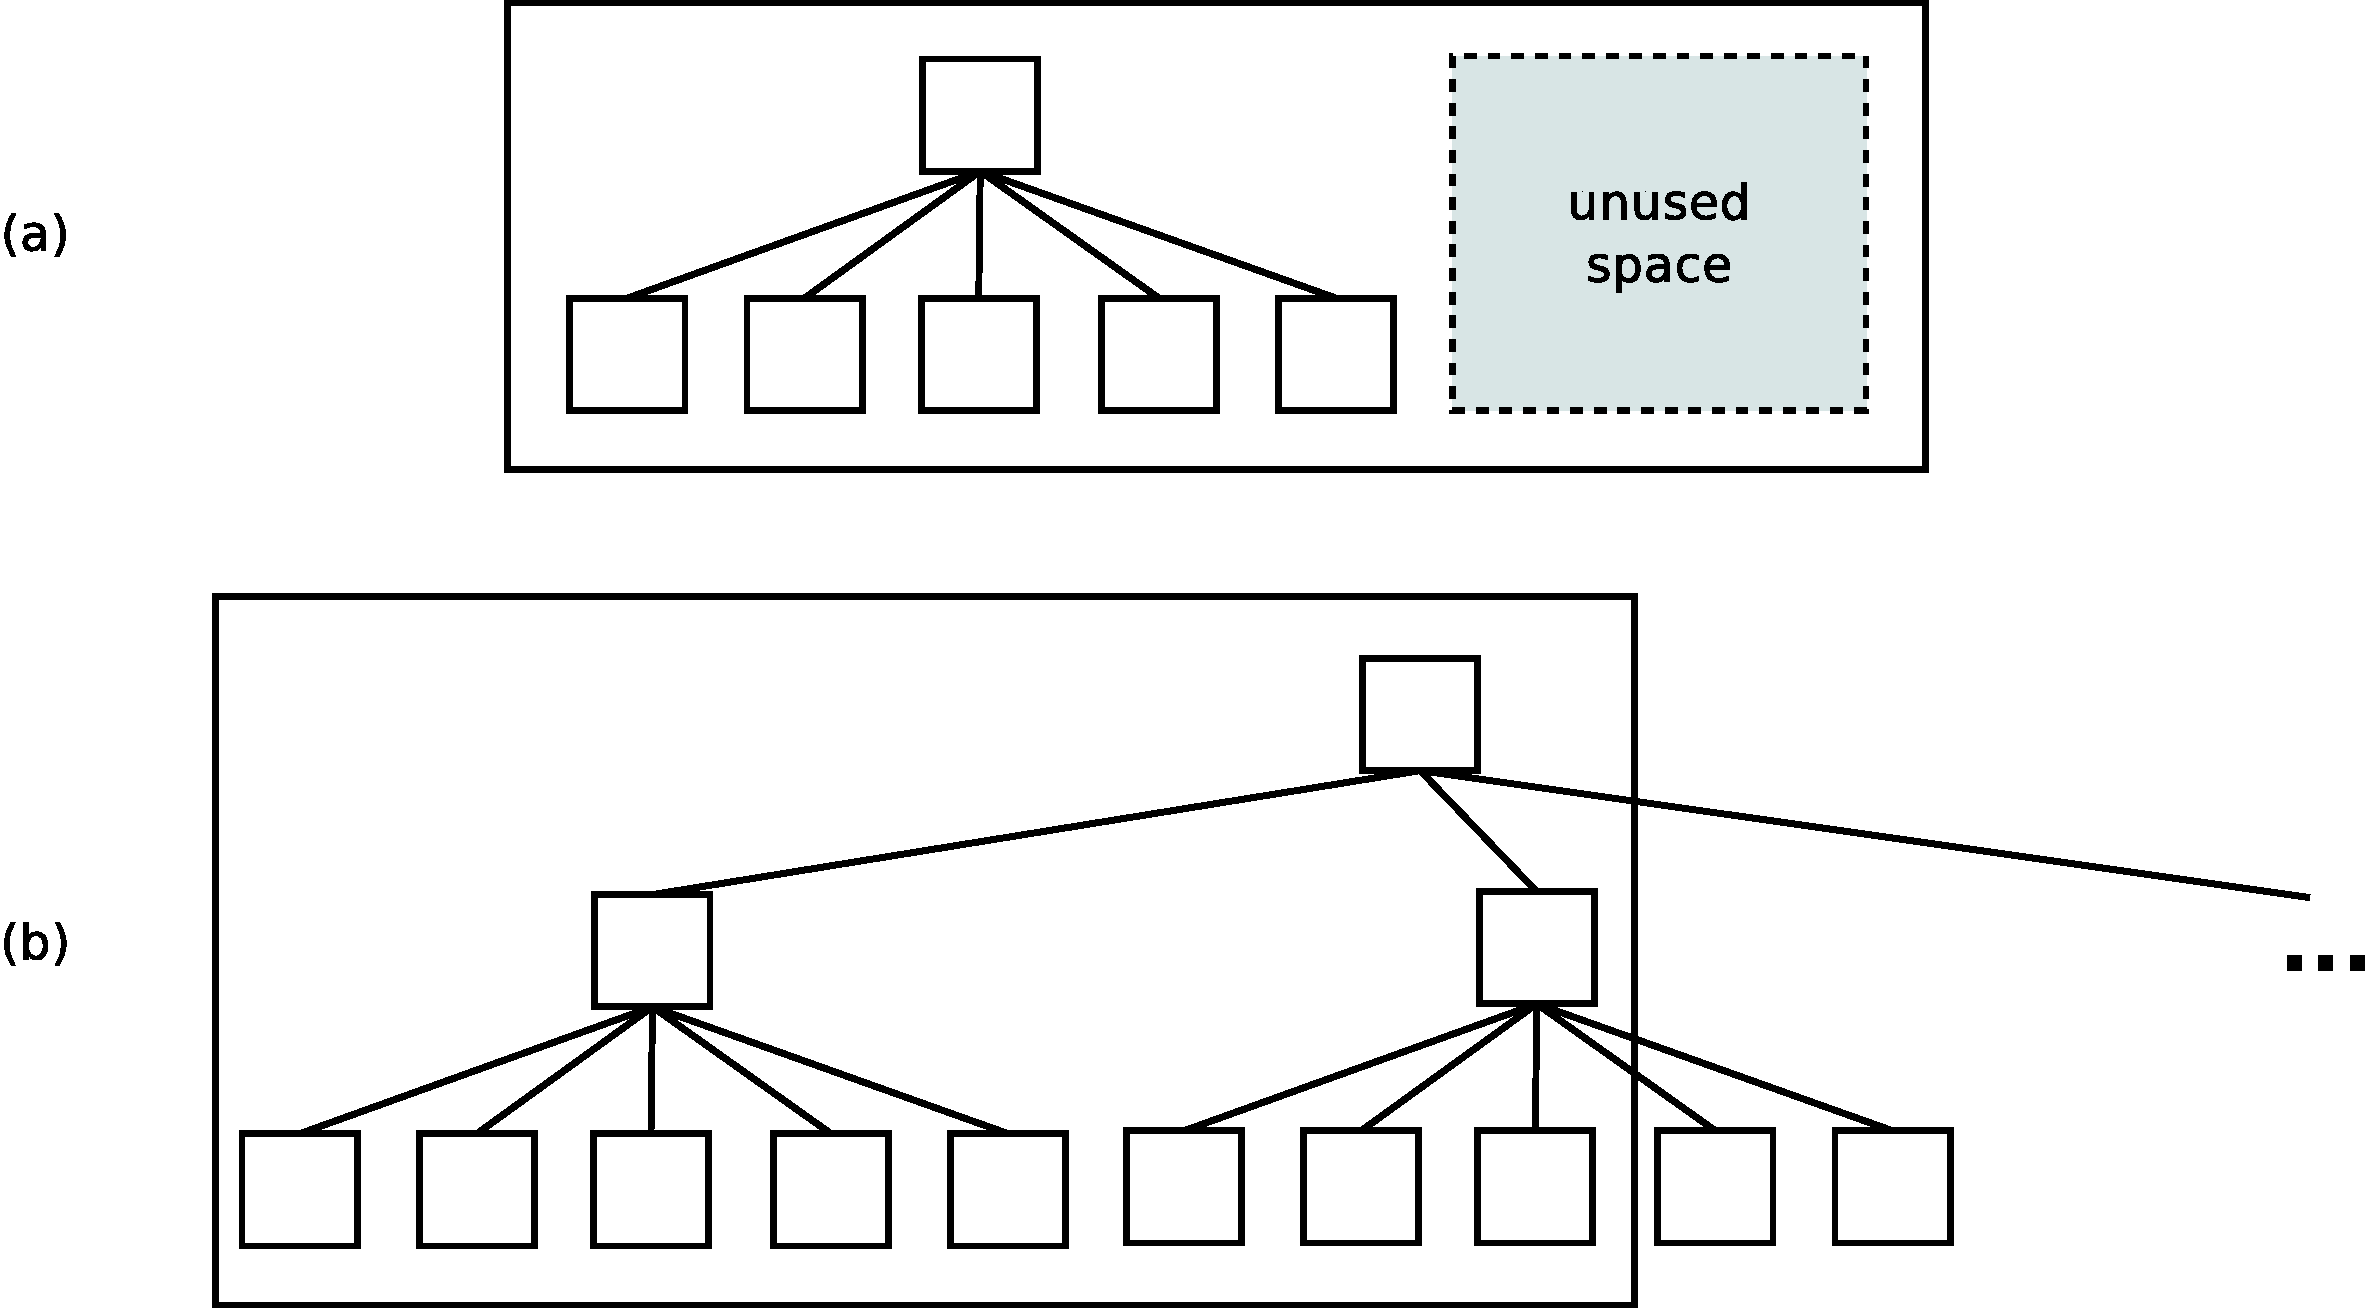
\includegraphics[width=300pt]{node_mismatch}
\end{center}
\caption{
(a) A two-level small tree that underflows the big node (b) Adding a third level to the tree in (a)
makes it overflow the big node. 
}
\label{fig:node_mismatch}
\end{figure}

We can approximate the cost of loading a small node into cache to be $c =
(T_{cm} + (w-1)\cdot T_{pf})$, where $T_{cm}$ is the cost of a cache miss and
$T_{pf}$ is cost of prefetching the next spatially contiguous cache line. In
modern processors, $T_{cm}$ is usually much larger than $T_{pf}$. This makes the
cost of searching through the small tree equal to $C = ch = c\cdot \log_b N$. From this expression, we 
observe that the cost of searching through the small tree grows as 
$\displaystyle O\left(\frac{b}{\log b}\right)$ with respect to the branching factor.

Hence, there is a tradeoff between space utilization and performance. As 
previously noted, this tradeoff is architecture dependent. So the best we can
do is empirically find the optimal value for $w$ that provides the desirable balance
between space utilization and performance. For the purposes of our project, we
only try to maximize performance because disks are cheap enough that for all practical purposes
disk space can be considered a free resource.

\usman Add a note saying that we produced this anaylsis in the attempt to experiment with the
result of the paper from which we took inspiration.
We tried to analytically predict the impact of the parameters, but in the end we have
realized that the dependence of the characteristics of the hardware was too strong,
and thus the only way to choose the parameters is experimentally.
To this end, at the end of the paper we run benchmarks to try to identify the
parameters and to analyze the accuracy of our theoretical intuition. 

\section{Adding Caching: cfB+ trees}
\subsection{Using Gaps for the Greater Good}
This far, we have illustrated how fpB+ trees store a small B+ tree in each big
node.
The strategy proposed for fpB+ trees is to fragment big nodes into smaller nodes
when the small trees
are mostly empty, and pack multiple big nodes in the same disk page.
Instead, when big nodes grow, the inverse strategy is applied and big nodes are
split and spread
across pages.

This process adds complexity to the implementation, and only guarantees that
pages are filled
homogeneously, not that space waste is minimized.
Indeed, when a big block the size of a page is split in half,
we can expect the former page to become half empty and the new one to become
half full.

We propose instead that a page always represent a single big node, and the space
gaps in the page
be exploited to cache database tuples.
Compared to the strategy for fpB+ trees, we avoid compressing big nodes,
resulting in an
even less efficient tree space usage.
However, we also exploit all the space which is not allocated to the tree to
store cached tuples,
so that almost no space is left unused.

This allows to return searched tuples which are in cache without the additional
overhead of reading a page from
the actual tuple storage.
The operating system tries to maintain pages which are accessed frequently in
memory for faster
access.
Also, pages belonging to the index are accessed more often than tuple pages,
because every operation
needs to walk a path in the index.
Therefore, caching tuples in the index has the double advantage of reducing the
likelihood
of a read to tuple page which is not in memory, and reducing the need for the
operating systems
to replace index pages in memory with tuple pages.
The same fact remains relevant for integrated database systems, which strongly
enforce the policy of keeping
index pages in memory.


\subsection{Patterns of Memory (Un)Usage}
We refer to the memory space necessary to store a small node as a \textit{slot}.
Each big node contains a fixed number $\sigma$ of slots, part of which will be
in use
as small nodes, while the rest will be available for cache (Figure
\ref{fig:inner_block}).
\begin{figure}[h]
\begin{center}
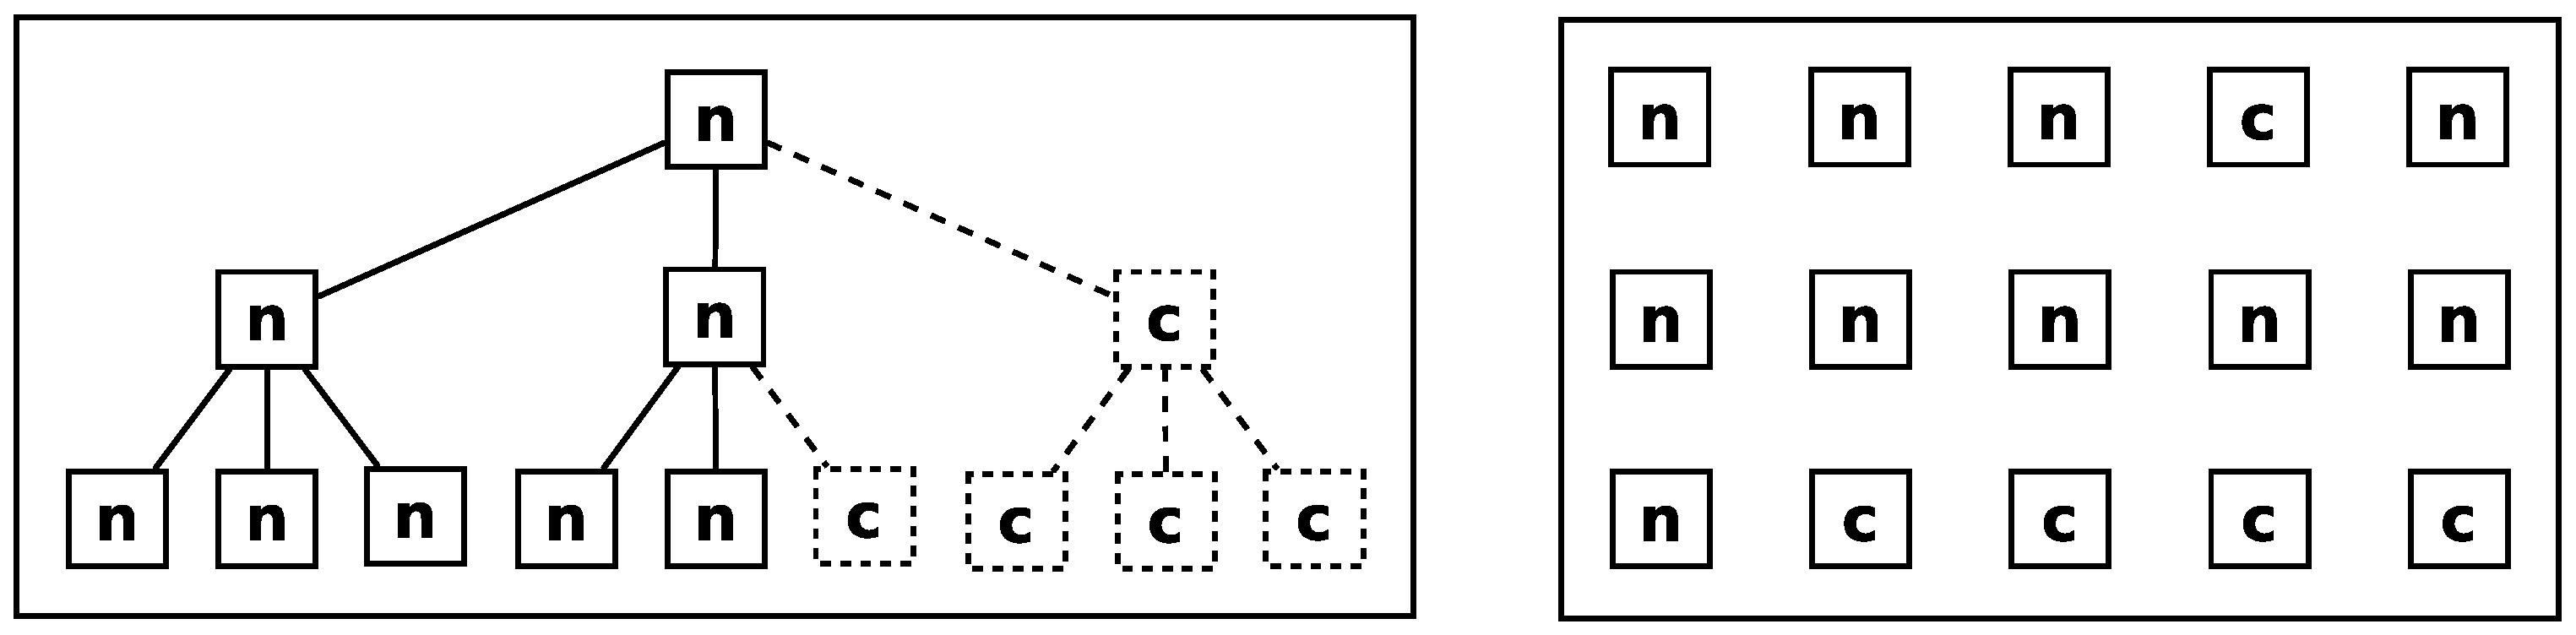
\includegraphics[width=350pt]{inner_block}
\end{center}
\caption{
The content of a big node.
On the left, a small tree as it is interpreted logically.
On the right, a small tree laid out in memory, with slots available for cache.
}
\label{fig:inner_block}
\end{figure}

In order to justify our choice to utilize unused slots as cache,
we recall the fact provided earlier that
B+ trees tend to be full at around 68\% of their capacity under standard
database loads \citep{Wu:2011}.
Thus, given that the tree should be fairly well balanced,
we expect to have $0.3 \sigma$ slots available for cache on average in leaf big
blocks.
As long as tuples are small enough to fit in a single slot,
we expect then to be able to cache around half of the tuples indexed in the
tree.
Otherwise, we can store a projection of the data, meaning a subset of the most
utilized fields for each entry,
and still read the disk storage if we don't find a field we are interested in.

Furthermore, unused slots are all the same size, and they are all located at an
integer multiple
of the slot size, making them easy to access and fast to read without much
overhead.


\subsection{Caching tuples}
An important fact to notice is that the pattern of insertions and removals
determines the shape of the tree;
therefore, the distribution of slots available for cache in memory is hard to
analyze.
Moreover, as items are inserted and removed, new nodes are also added and
removed;
correspondingly, slots that were once available are allocated to the
tree and become unavailable to the cache, and vice-versa.
This is evident even from Figure \ref{fig:inner_block}, which illustrates that
slots available for cache are sparse in the big node.

It is apparent then that the scenario is reminescent of that of a hash table.
In fact, we can consider the function that allocates slots to the small tree to
be an adversary
hash function grabbing and releasing cache slots outside of the control of
our cache system.
We can then interpret the problem as that of finding a suitable hash system
able to perform well under the external influence of node assignments.
To the best of our knowledge, there has not been relevant research
to address this problem, so we approach it from the perspective that there
is no way to optimize our strategy from a theoretial perspective.

Intuitively, a candidate hashing strategy can take inspiration from open
addressing.
Conside a big node $B$ on the path to the leaf that points to tuple $\tau$.
With open addressing, we insert by repeatedly hashing the key for $\tau$ to a
slot in $B$,
till we find a slot that is available for cache and has room for one more cache
entry.
Similarly, we search by repeatedly hashing the key for $\tau$ till we either
find
a cache slot containing $\tau$, we find a cache slot with room for more entries,
or we have probed every slot in the big node.
With this scheme, a cache slot converted to a tree node effectively results
in the cache entries at that slot being evicted from cache.

Notice that, unlike for the case of traditional open addressing, we do not
assume an item is not cached
if we hash to a slot that has available room but does not contain it.
That is because otherwise, when a tree node is released and made available from
cache, we would risk
invalidating parts of the cache.
In spite of the fact that we may need to probe all slots often, performance
should not degrade in practice
thanks to prefetching.
If we employ linear probing, the processor will fetch the next slots as we
process the current one,
resulting in an almost negligible cost to access the entire big node.
That is especially the case for modern processors, which have data L1 cache in
the order of tens of KB,
so the entire big node can be prefected to near processor cache.

Inconveniently, the efficiency of open addressing with linear probing decays
very rapidly as the fill factor
of the big node increases, canceling the advantages of hashing compared to
linearly scanning all slots.
Also, strategies that are more theoretically appealing such as cuckoo and
hopscotch hashing
would not fit the problem conveniently, as displacing a slot used as a node
would require to update all references
to it from other nodes.

A possible improvement could come from implementing a coalesced hashing strategy
\citep{Vitter:1987}.
Coalesced hashing unites chaining with open addressing by storing chains of
items that would
share the same bucket sparsely throughout the table but connected by pointers.
This reduces clustering, while maintaining the ability to use small, fixed-sized
slots as opposed to growing chains.
In the worst case with a long, sparse chain the behavior of coalesced hashing
would approximated a linear
scan in random order, voiding the benefits of prefetching.
Therefore, we leave the problem of improving over open addressing for a future
implementation.

Another problem that we leave open to further investigation is eviction order
when the cache is full.
As we previously stated, some evictions will necessarily happen when a cache
slot is upgraded to a node slot.
However, in many typical database access scenarios, searches largely dominate
insertions and deletions.
Therefore, we would like to have an eviction policy for the case of long series
of queries, for instance LRU.
The main difficulty of implementing a least-recently accessed logic would be the
reduction
in available cache space due to the need to store additional information for
access time,
or the need to frequently rearrange cached items to maintain them ordered by
access time.
Given that slots are already of comparably or lesser sized than an average
tuple, it would be a challenge
to add metainformation, but it is conceivable that a smart rearrangement process
could be fruitful.

\section{Experimental Results}

\subsection{Implementations}
We produced three implementations: a basic, unoptimized B+ tree as control, an
fpB+ tree and a cfB+ tree.
The fpB+ tree follows the same design guidelines that we laid down in this paper
for cfB+ trees,
so that the two differ solely by the presence or absence of our data caching
strategy.
This delegates the task of maintaining the first few levels of the tree in
memory to the system page cache,
a choice that can be easily reversed by adding a memory management framework.

Slots in big nodes are allocated/deallocated to/from the tree with an elementary
linear probing strategy,
and small nodes are also searched linearly.
Processor cache is instrumental in making these operations efficient
independently from their asymptotic performance.

Big nodes are managed lazily, so that insertions are appended after the last
one, and removals results in gaps.
When the number of gaps increases to equal the number of used blocks, we compact
the entire structure.
This yields an amortized constant cost, because only one block is moved for
every block that was deleted.
Also, it ensure that the total space occupied by the structure is always
asymptotically linear in the number
of big nodes being actively used.

We support only the basic query operations, leaving the more complex range
queries to a future improvement.
We notice however that, just like fpB+ trees, cfB+ trees can be augmented with
jump pointers to that end.
All the leaves with values would be stored outside the tree in a sorted,
contiguous fashion.
Jump pointers would be maintained in the tree, and a search to the leftmost
element in a range would be performed.
Then, it would be sufficient to scan the leaves rightwards till the right
boundary of the range is exceeded.
Again, due to the contiguous nature of the leaves, prefetching would help the
performance of the operation.

A problem that could be helped by future work is reducing the implementation
complexity for the cfB+ tree.
The two different granularities at which the structure exist, big tree with big
nodes and small trees with small nodes
at each big node, results in a high complexity burden on the developer.
The most complex operation is splitting, as it recurses at both granularities,
intertwining insertions in parents
and copies of children with the need to keep all relative likes between nodes
updated throughout the move.
Thus, it would benefit from a cleaner interface between the operations than the
one we designed under
time constraints. 
This complexity connected with keeping ancestors-descendants coherency at
different granularities
is also what prompted us not to add additional granularities to exploit the
three levels of processor cache
or to adapt the structure for cache-obliviousness.


\subsection{Benchmarks}
For all benchmarks we used a Linux 2.6.39 system based on an Intel Core i7 920
with 4 GB of RAM.
All code was written in the C language, and compiled with gcc version 4.6.1 with
level-3 optimizations enabled.

\begin{figure}[h]
\begin{center}
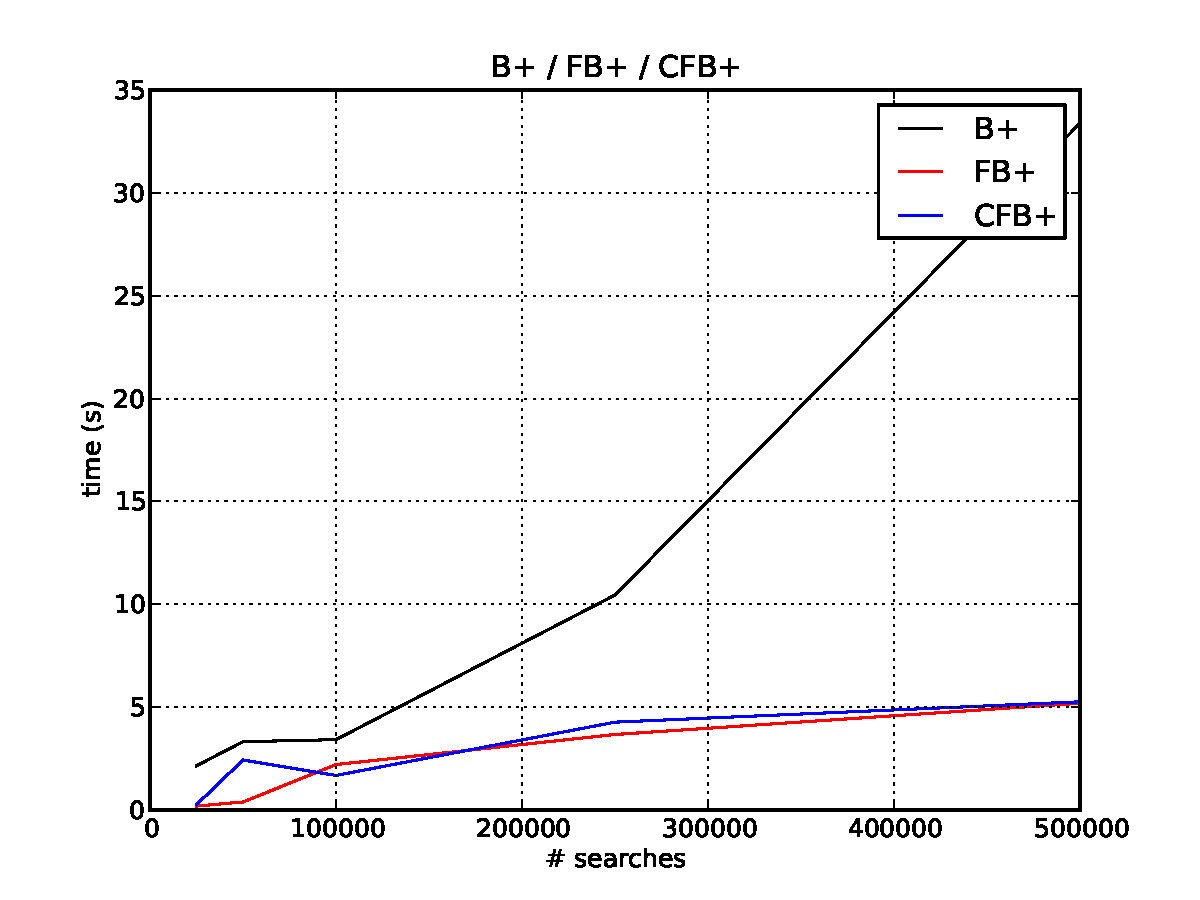
\includegraphics[width=280pt]{base}
\end{center}
\caption{
Comparison of performance of B+, fpB+, cfB+ trees.
Database entries are not fetched from disk, which cancels the
advantage of cfB+ trees against fpB+ trees.
The query speedup so obtain serves the purpose
of illustrating the behavior of fractal trees versus basic trees as the number
of queries increases.}
\label{fig:base}
\end{figure}

We started with a preliminary benchmark, aimed at comparing basic B+ tree
performance against fractal B+ tree performance. showing an improvement
The results, illustrated in Figure \ref{fig:base}, show a performance increase
above 5x.
For this benchmark, we tested only data structure operations to better show the
difference in performance
achieve by the fractal structure alone. When a key was searched in the index structure, the
corresponding tuple was not fetched from disk. At the same time, the relative performance of the
fpB+ tree and the cfB+ tree also indicates that the overhead of using open addressing to probe the cache
while perfoming a search is negligible. We also noted similar performance increase of upto 3x for 
an insert workload.

\begin{figure}[H]
\begin{center}
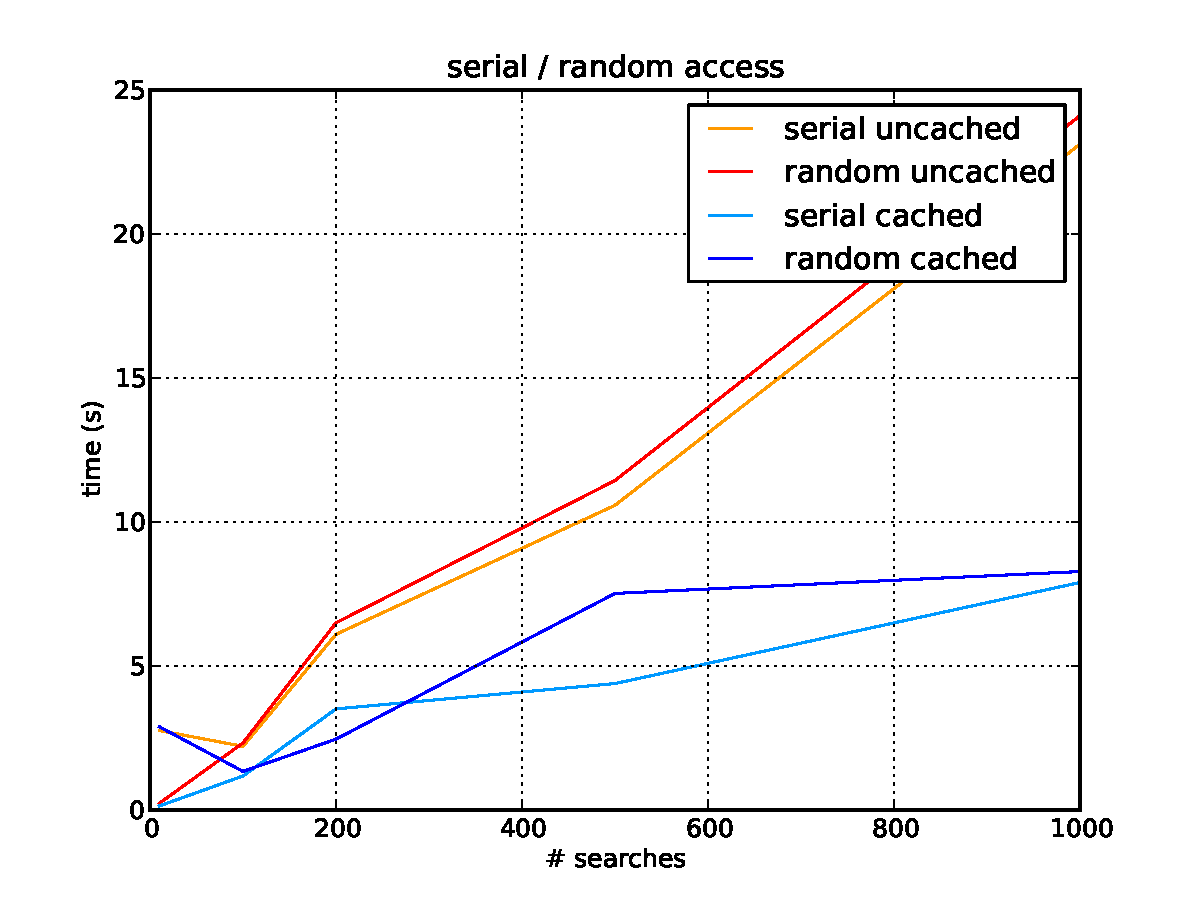
\includegraphics[width=280pt]{combs}
\end{center}
\caption{
Comparison of performance of fpB+ trees vs cfB+ trees for sequential searches
and random searches.
The total number of items in the trees is 2000, and the cache was pre-heated by
1000 random reads.
}
\label{fig:combs}
\end{figure}

We proceeded to recreate the realistic case where RAM size is negligible
compared to database size by
forcing the operating system not to cache database entry pages.
This is the case most of the times in databases, and this is where our cfB+
trees excel.
Figure \ref{fig:combs} shows the results of querying items serially and randomly
both for fpB+ and cfB+ trees.
The cfB+ trees achieve a performance increase of approximately 5x compared to
the fpB+ trees. We note that searching randomly for keys in the cfB+ tree becomes 
faster as the number of searches increases, while the opposite can be said for sequential searches. 
We believe that in the case of searching for keys randomly, the expected hit rate should increase 
as we search for more keys, because as the cache fills the probability of a cache hit increases. 
In the case of sequential searches, however, we never look up the same key twice so we never experience any 
cache miss abosorption.

Finally, we tested a set of realistic parameters for the tree, showing how
performance changes with the number
of cache hits in the cfB+ tree. All parameters that are small integers multiples
of page size and cache line
size perform similarly well, with larger branching factors enjoying better performance due to 
smaller tree heights.
The results are in Figure \ref{fig:cachehits1} and Figure \ref{fig:cachehits2}.
In real-world applications, databases tend to be queried the most often for
recent values,
so we would expect the number of cache hits to be high.
In the worst case, when there are no cache hits, we pay a small overhead penalty
to support the cache.
However, when all searches are hits, cfB+ trees are 35x faster than fpB+ trees.

\begin{figure}[h]
\begin{tabular}{l l}
\includegraphics[width=250pt]{4096_64_6} &
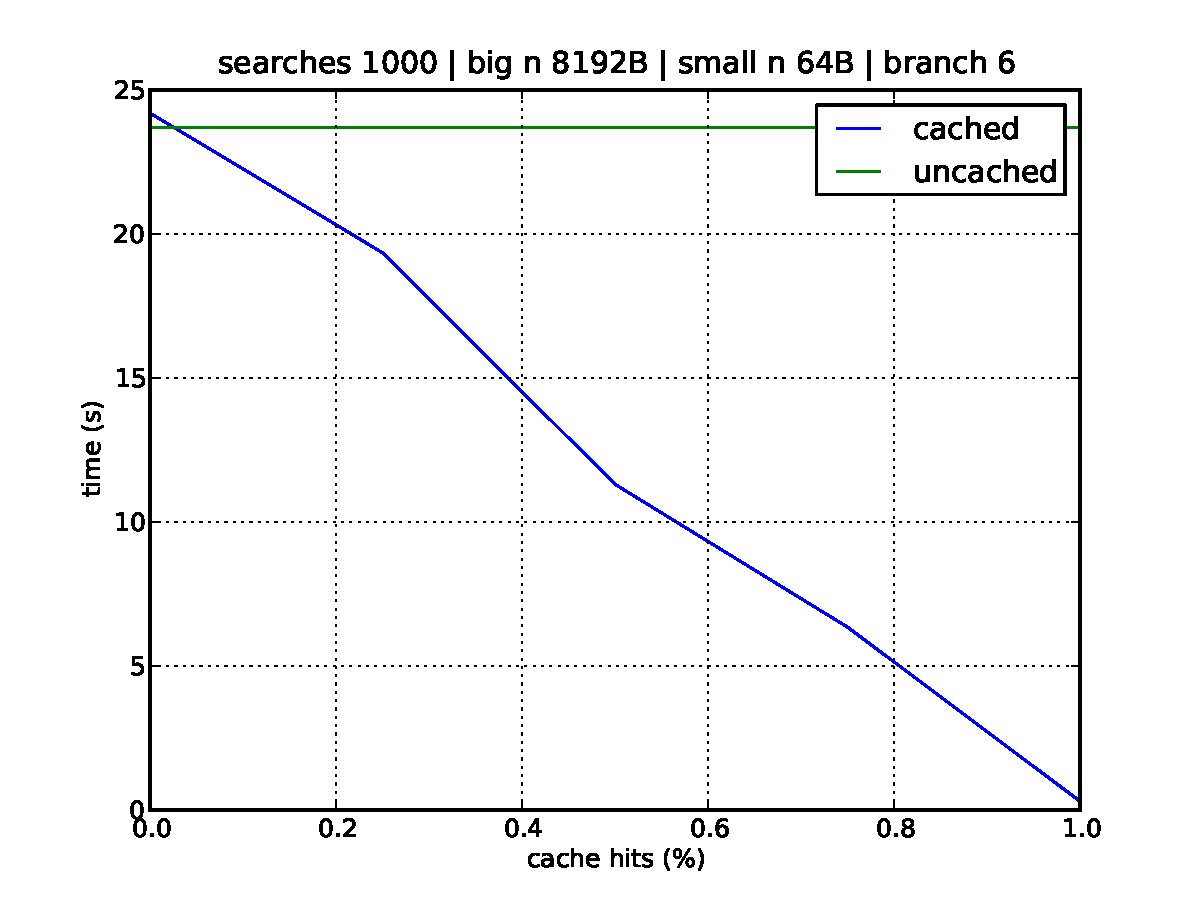
\includegraphics[width=250pt]{8192_64_6} \\
\includegraphics[width=250pt]{4096_128_12} &
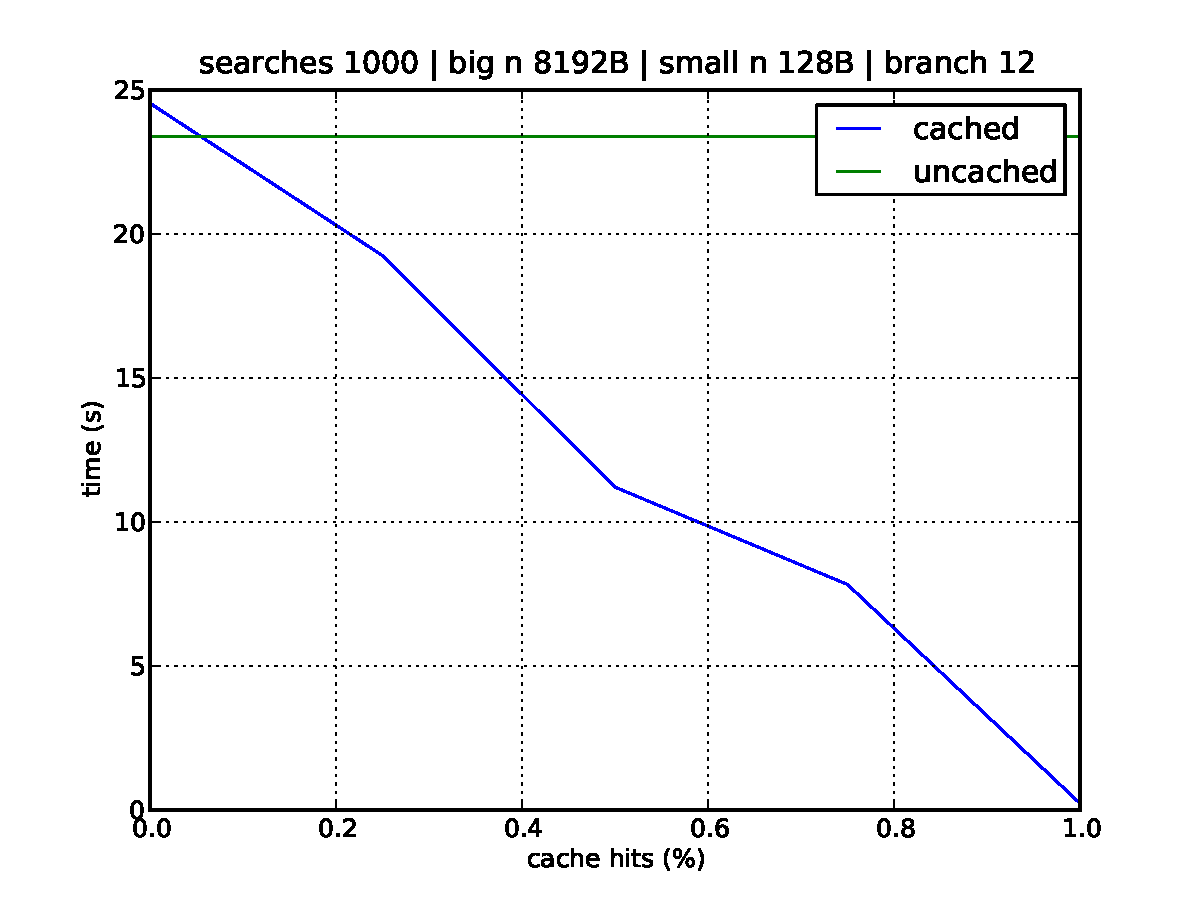
\includegraphics[width=250pt]{8192_128_12} \\
\end{tabular}
\caption{
Comparison of performance of fpB+ trees vs cfB+ trees for various parameters,
matching integer multiples of the page and cache line boundaries.
}
\label{fig:cachehits1}
\end{figure}

\begin{figure}[h]
\begin{tabular}{l l}
\includegraphics[width=250pt]{4096_256_24} &
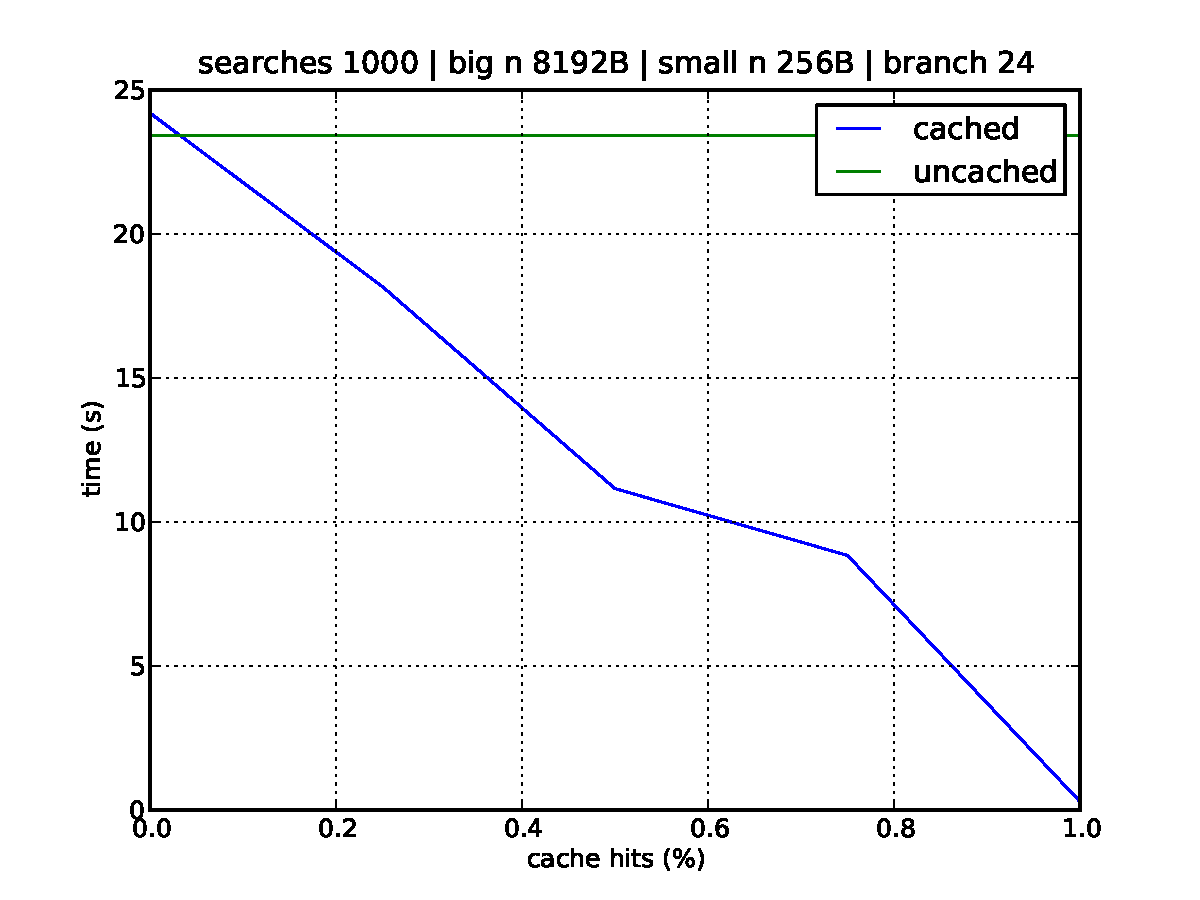
\includegraphics[width=250pt]{8192_256_24} \\
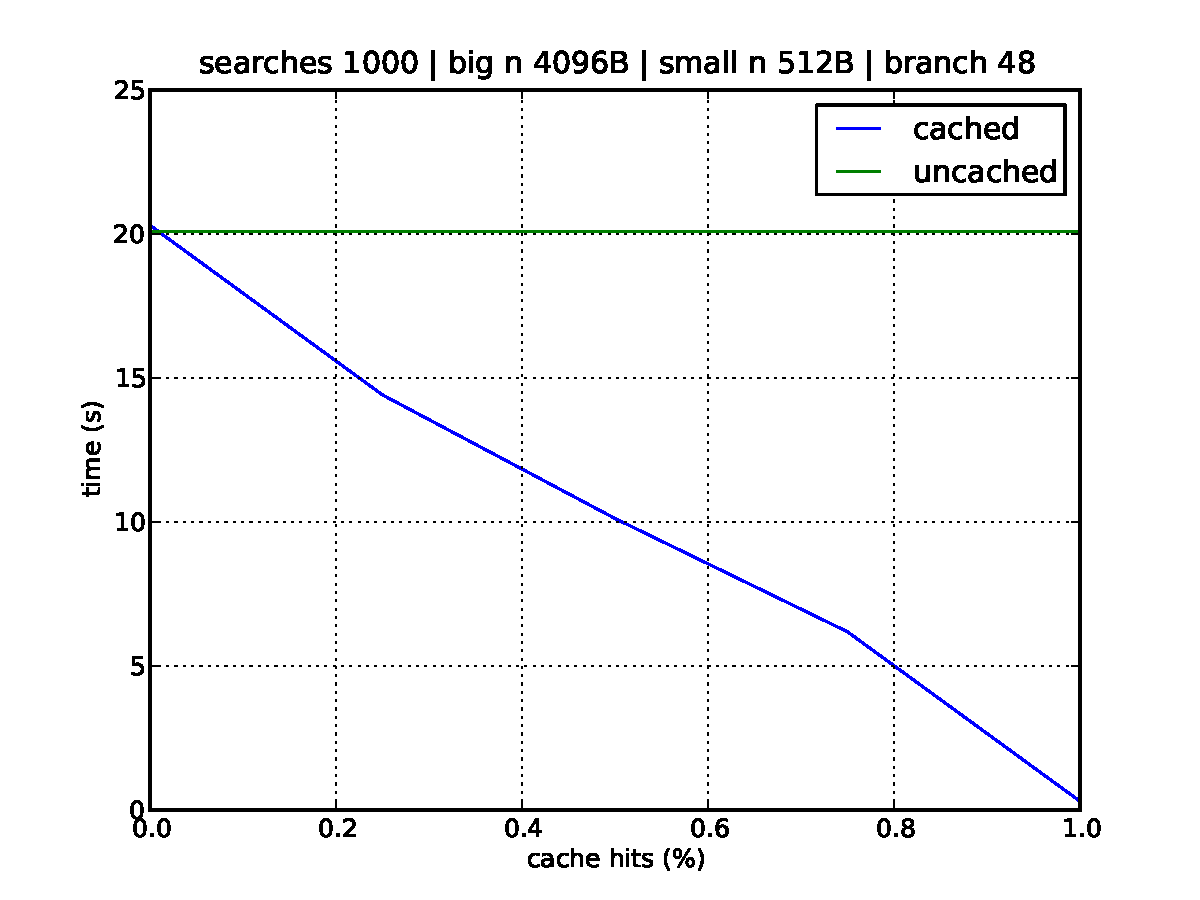
\includegraphics[width=250pt]{4096_512_48} &
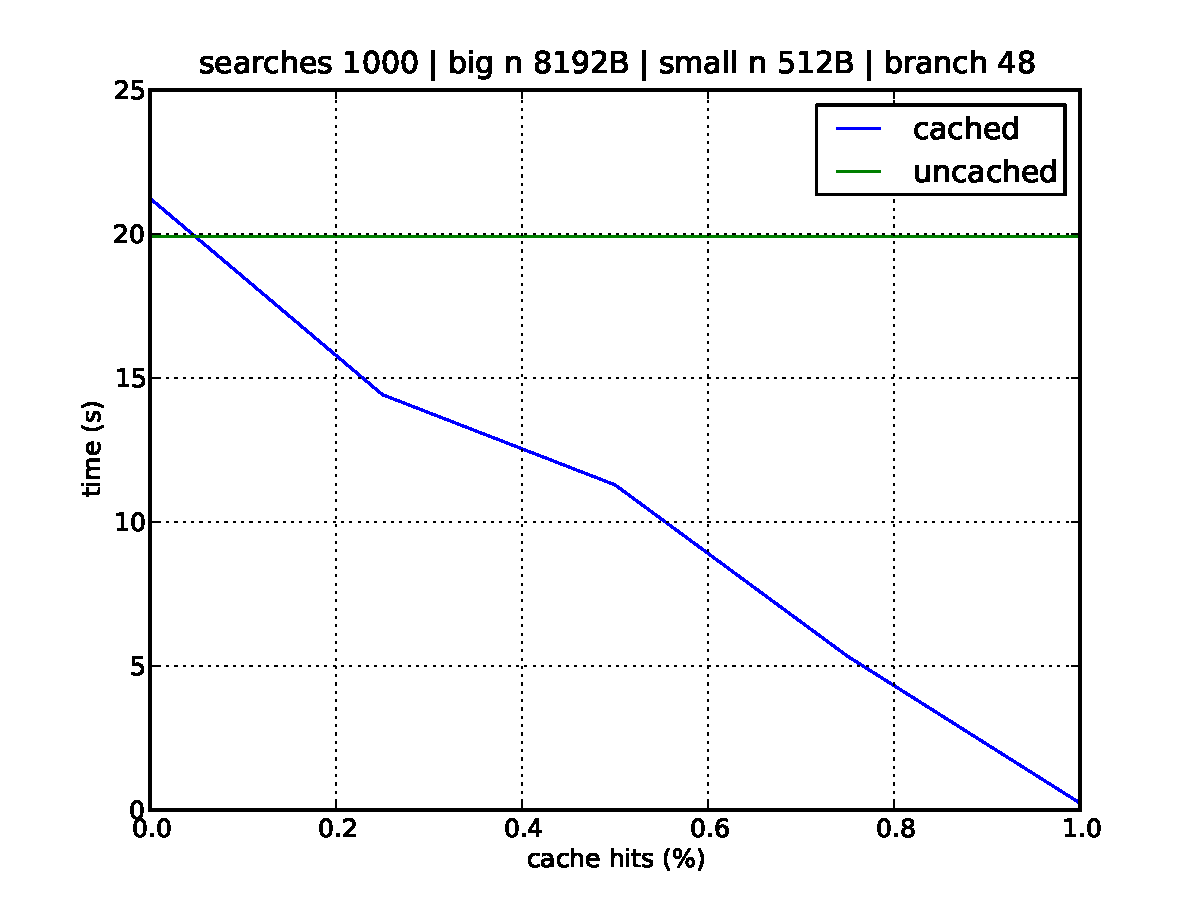
\includegraphics[width=250pt]{8192_512_48} \\
\end{tabular}
\caption{
Comparison of performance of fpB+ trees vs cfB+ trees for various parameters,
matching integer multiples of the page and cache line boundaries.
}
\label{fig:cachehits2}
\end{figure}

\section{Conclusions}
We presented a new data structure, the cfB+ tree, which simplifies fpB+ trees by
reducing the need for tree reorganization,
while taking advantage of temporarily unused memory locations as database tuple
caches.
We discussed challenges of the implementation, as well as problems that remain
open,
such as improving upon the caching strategy and defining an efficient cache
eviction policy.
Finally, we showed that, cfB+ trees improve upon fpB+ trees by a factor ranging
from -1.2 to 35 depending on the number of cache hits. For a typical database
work load, we found the cache hit rates to be around YY\% which have us a YYx
improvement.

\small

\bibliographystyle{apalike}
\bibliography{final}


\end{document}
